\graphicspath{{../bidithi/pic/}}
\begin{center}
	\textbf{\Large\color{toancuabi}MỘT SỐ BÀI TOÁN VỀ TỔ HỢP ĐẾM (COUNTING) TRONG KỲ THI HỌC SINH GIỎI CẤP TIỂU HỌC}
\end{center}
Trong chương trình phổ thông của Việt Nam, toán tổ hợp đếm được giới thiệu ở cấp THPT. Tuy nhiên trong một số cuộc thi học sinh giỏi toán dành cho cấp tiểu học và đầu cấp PTCS thì phần tổ hợp đếm đã được đưa vào nội dung bài thi khá nhiều, ví dụ như một số cuộc thi khá phổ biến ở Việt Nam hiện nay như IMAS (International Mathematics Assessment), Apmops (The Asia Pacific Mathematical Olympiad for Primary Schools), IMSO (The International Mathematics and Science Olympiad)...
\vskip 0.1cm
Trong bài viết này chúng ta cùng làm quen với một số bài toán về đếm tổ hợp trong một số cuộc thi học sinh giỏi cấp tiểu học và lớp $6$ THCS.
\vskip 0.1cm
Trước hết chúng ta làm quen với một số khái niệm cơ bản trong phần toán tổ hợp đếm.
\begin{multicols}{2}
	\textbf{Quy tắc cộng, quy tắc nhân:} Quy tắc cộng và quy tắc nhân là hai quy tắc đếm cơ bản, có nội dung có thể được mô tả như sau:
	\vskip 0.1cm
	Có hai công việc gọi là Job $1$ và Job $2$ (có thể mở rộng ra nhiều hơn $2$ công việc) được thực hiện một cách độc lập nhau. Có $m$ cách thực hiện Job $1$ và $n$ cách thực hiện Job $2$, khi đó hai quy tắc đếm cơ bản được phát biểu như sau:
	\vskip 0.1cm
	\textbf{Quy tắc cộng:} Có $m+n$ cách để thực hiện Job $1$ hoặc Job $2$.
	\begin{figure}[H]
		\centering
		\vspace*{-10pt}
		\captionsetup{labelformat=empty, justification=centering}
		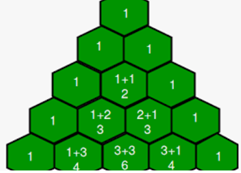
\includegraphics[width=0.47\textwidth]{1}
		\caption{\small\textit{Quy tắc cộng trong tam giác Pascal.}}
		\vspace*{-5pt}
	\end{figure}
	\textbf{Quy tắc nhân:} Có $m\times n$ cách để thực hiện Job1 và Job2 (thực hiện cả hai công việc).
	\begin{figure}[H]
		\centering
		\vspace*{5pt}
		\captionsetup{labelformat=empty, justification=centering}
		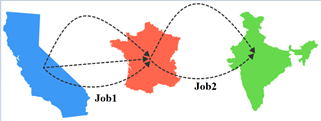
\includegraphics[width=0.48\textwidth]{2}
		\caption{\small\textit{Quy tắc nhân trong bài toán đếm đường đi.}}
		\vspace*{-10pt}
	\end{figure}
\textbf{Giai thừa:} của $n$ là số cách sắp xếp thứ tự của n phần tử trong một tập hợp, được ký hiệu là $n!$ và có công thức là: $n!=1\times 2\times 3\times \ldots\times n $.
\vskip 0.1cm
Ghi chú: $0!=1$
	\begin{figure}[H]
	\centering
	\vspace*{-5pt}
	\captionsetup{labelformat=empty, justification=centering}
	
\includegraphics[width=0.48\textwidth]{3}
	\vspace*{-15pt}
\end{figure}
\end{multicols}
\textbf{Hoán vị (Permutation):} Có $n$ người và chỉ có $k$ cái ghế trên một hàng ($k\le n$), ta cần xếp đủ $k$ người từ nhóm $n$ người vào $k$ cái ghế. Khi đó số cách xếp gọi là hoán vị và ký hiệu là:
\begin{align*}
	P(n,k)=n\times(n-1)\times(n-2)\times\ldots\times(n-k+1)= \frac{n!}{(n-k)!} 
\end{align*}
\begin{multicols}{2}
	Trong trường hợp có $n$ người và có đúng $n$ cái ghế khi đó ta có số cách sắp xếp $n$ người này chính là định nghĩa của $n!$ (số cách sắp xếp các phần tử của một tập hợp $n$ phần tử): $P(n,n)=n!$
	\begin{figure}[H]
		\centering
%		\vspace*{pt}
		\captionsetup{labelformat=empty, justification=centering}
		
\includegraphics[width=0.48\textwidth]{4}
		\vspace*{-10pt}
	\end{figure}
\end{multicols}
	\textbf{Hoán vị vòng tròn (Circular Permutation):} Xung quanh một bàn tròn có $n$ người ngồi. Hai hoán vị được coi là như nhau nếu chúng có thể chồng khít vào nhau bằng phép xuay. Số cách sắp xếp $n$ người xung quanh môt cái bàn tròn cố định là: (\textit{cố định: có nghĩa là ta không thể nhấc nó ra để lật ngược lại được})
	\begin{align*}
		P_n=(n-1)!
	\end{align*}
	Số là $(n-1)!$ thay vì $n!$ vì có $n$ cách xoay bàn và $n$ hoán vị do xoay bàn từ $1$ vị trí là như nhau.
	\begin{figure}[H]
		\centering
		\vspace*{-5pt}
		\captionsetup{labelformat=empty, justification=centering}
		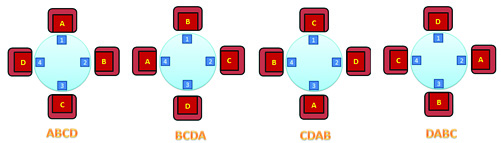
\includegraphics[width=0.48\textwidth]{5}
		\caption{\small\textit{Hoán vị vòng tròn $4$ người ngồi xung quanh một cái bàn hình tròn.}}
		\vspace*{-15pt}
	\end{figure}
\textbf{Tổ hợp (Combonation):}  Đếm số cách để chọn $k$ người từ một nhóm $n$ người là một trong những bài toán tổ hợp đếm cơ bản, và nó được gọi bằng một cái tên đặc biệt: TỔ HỢP và được ký hiệu  $C(n,k)$; $C_n^k$ và có công thức là:
\begin{align*}
	C_n^k=C(n,k)&=\frac{P(n,k)}{k!} = \frac{n\times(n-1)\times(n-2)\times\ldots \times(n-k+1)}{k!}\\
	& = \frac{n!}{k!\times(n-k)!}
\end{align*}
\begin{multicols}{2}
	\textbf{Bài toán số $1$: (IMAS)}
	\vskip 0.1cm
	Sơ đồ dưới đây gồm nhiều tam giác vuông cân.
	\vskip 0.1cm
	Có bao nhiêu cách một con kiến có thể đi từ $A$ đến $C$ nếu nó chỉ được phép di chuyển lên trên, sang phải hay theo đường chéo? 
	\begin{figure}[H]
		\centering
		\vspace*{-5pt}
		\captionsetup{labelformat=empty, justification=centering}
		
\includegraphics[width=0.4\textwidth]{6}
		%	\caption{\small\textit{Hoán vị vòng tròn $4$ người ngồi xung quanh một cái bàn hình tròn.}}
		\vspace*{-15pt}
	\end{figure}
\end{multicols}
\textbf{Phân tích bài toán:} Tại mỗi điểm nút trên hình vẽ, số cách đi từ $A$ đến nó sẽ bằng tổng số cách đi từ $A$ đến các điểm nút ngay đằng trước nó theo chiều mũi tên được phép đi (phải, lên trên và đi chéo).
\begin{multicols}{2}
	\begin{figure}[H]
		\centering
		\vspace*{-5pt}
		\captionsetup{labelformat=empty, justification=centering}
		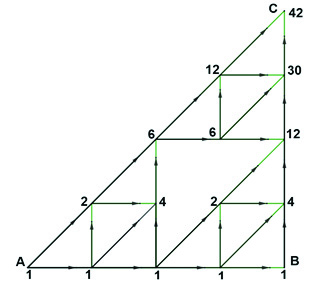
\includegraphics[width=0.4\textwidth]{7}
		%	\caption{\small\textit{Hoán vị vòng tròn $4$ người ngồi xung quanh một cái bàn hình tròn.}}
		\vspace*{-15pt}
	\end{figure}
	Vậy nên ta có để điền mũi tên hướng đi và áp dụng quy tắc cộng để giải quyết các bài toán dạng này.
	\vskip 0.1cm
	\textit{Lời giải}: Theo quy tắc cộng thể hiện trên hình vẽ bên dưới ta có tổng số cách đi từ $A$ đến $C$ là $42$.
\end{multicols}

\textbf{Bài toán số $2$: (IMAS)}
\vskip 0.1cm
$8$ ký tự $2,0,1,5,I,M,A,S$ được xếp trên $1$ hàng. Hỏi có bao nhiêu cách xếp sao cho các chữ số đứng đằng trước các chữ cái, chữ số $0$ không đứng đầu tiên.
\vskip 0.1cm
\textit{Lời giải.}
Có $8$ vị trí để xếp $8$ ký tự, các chữ số đứng đằng trước các chữ cái nên $4$ vị trí đầu tiên là các chữ số và $4$ vị trí sau cùng. Ta thực hiện $2$ công việc là xếp chữ số và xếp chữ cái:
\vskip 0.1cm
+ Có $3\times3\times2\times1=18$ cách xếp các chữ số (chữ số $0$ không đứng ở đầu nên vị trí đầu chỉ có $3$ cách chọn chữ số).
\vskip 0.1cm
+ Có $4\times3\times2\times1=4!=24$ cách xếp $4$ chữ cái.
\vskip 0.1cm
Theo quy tắc nhân (hai quy tắc cơ bản trong đếm tổ hợp là quy tắc cộng và quy tắc nhân) ta có số cách xếp $8$ ký tự là: $18\times24=432$.
\vskip 0.1cm
(Ta có thể lập luận: ta thực hiện $3$ công việc theo thứ tự là Job $1$ là viết chữ số đầu tiên, Job $2$ là viết $3$ chữ số tiếp theo, Job $3$ là viết $4$ chữ cái, và theo quy tắc nhân ta có kết quả là: $P(3,1)\times P(3,3)\times P(4,4)=3\times3!\times4!=432$)
\vskip 0.1cm
Mở rộng bài toán số $2$, các bạn thử sức với bài toán số $3$ nhé.
\vskip 0.1cm
\textbf{Bài toán số $3$:}
\vskip 0.1cm
$8$ ký tự $2,0,1,5,I,M,A,S$ được xếp trên $1$ hàng. Hỏi có bao nhiêu cách xếp thỏa mãn một trong các điều kiện sau:
\vskip 0.1cm
$a)$ Không có hai chữ cái nào đứng cạnh nhau.
\vskip 0.1cm
$b)$ Chữ số $0$ nằm giữa hai chữ cái $I$ và $S$.
\vskip 0.1cm
$c)$ Chữ số $0$ và chữ số $1$ không đứng cạnh nhau.
\vskip 0.1cm
$d)$ $4$ chữ cái luôn đứng cạnh nhau.
\vskip 0.1cm
\textbf{Bài toán số $4$: (IMAS)}
\vskip 0.1cm
Có bao nhiêu số có $3$ chữ số không chứa chữ số $3$ và chia hết cho $3$.
\vskip 0.1cm
\textbf{Phân tích bài toán:}
\vskip 0.1cm
Gọi số có $3$ chữ số là $\overline{abc}$:
\begin{multicols}{2}
	Thử từ số nhỏ để tìm quy luật:
	\begin{align*}
		&102, 105, 108\\
		&111, 114, 117\\
		&120, 126, 129\\
		&132, 135, 138\\
		&141, 144, 147\\
		&150, 156, 159...
	\end{align*}
	Ta nhận thấy chữ số $c$ lặp theo nhóm $(2,5,8)$, $(1,4,7)$, $(0,6,9)$ và mỗi nhóm này xuất hiện phụ thuộc vào số dư chi $3$ của số $\overline{ab}$ từ đó ta có lời giải như sau:
\vskip 0.1cm
\textit{Lời giải}
\vskip 0.1cm
Nếu $\overline{ab}$ chia $3$ dư $0$ ta có $3$ cách chọn $c=\{0,6,7\}$
\vskip 0.1cm
Nếu $\overline{ab}$ chia $3$ dư $1$ ta có $3$ cách chọn $c=\{2,5,8\}$
\vskip 0.1cm
Nếu $\overline{ab}$ chia $3$ dư $2$ ta có $3$ cách chọn $c=\{1,4,7\}$
\vskip 0.1cm
Vậy mỗi số $\overline{ab}$ ta luôn có $3$ cách chọn chữ số $c$.
\vskip 0.1cm
Ta có $9\times 10$ cách tạo ra số $\overline{ab}$.
\vskip 0.1cm
Vậy số số có $3$ chữ số không chứa chữ số $3$ và chia hết cho $3$ là: $9\times10\times3=270$ (số);
\end{multicols}
\vskip 0.1cm
\textbf{Bài toán số $5$: (APMOPS)}
\vskip 0.1cm
Mỗi cạnh của hình ngũ giác có cạnh $a,b,c,d,e$ tương ứng được tô bằng một trong $3$ mầu xanh, đỏ, vàng. Hỏi có bao nhiêu cách tô mầu cách cạnh của hình ngũ giác này sao cho không có $2$ cạnh nào kề nhau có cùng mầu.
\begin{multicols}{2}
	\begin{figure}[H]
		\centering
		\vspace*{-10pt}
		\captionsetup{labelformat=empty, justification=centering}
		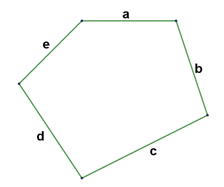
\includegraphics[width=0.4\textwidth]{8}
		%	\caption{\small\textit{Hoán vị vòng tròn $4$ người ngồi xung quanh một cái bàn hình tròn.}}
		\vspace*{-5pt}
	\end{figure}
	\textbf{Phân tích bài toán:} Nếu ta tô thứ tự $a,b,c,d,e$ thì $a$ và $b$ có tương ứng $3$ và $2$ cách tô. Đến tô $c$ thông thường sẽ có $2$ cách tô, $d$ cũng $2$ cách tô, nhưng nếu như vậy thì $e$ sẽ không xác định được số cách tô vì nó phụ thuộc vào $2$ cạnh $a$ và $d$, bởi vậy ta cần xét đến mầu cụ thể của $c$ cũng như của $d$ để tính được số cách tô mầu $c$. Vậy ta có thể tiếp cận bài toán bằng hai cách sau đây.
\vskip 0.1cm
\textit{Lời giải $1$:}
\vskip 0.1cm
Tô $a$, có $3$ cách tô, tô $b$, có $2$ cách tô.
\vskip 0.1cm
Tô $c$:
\vskip 0.1cm
\textbf{Trường hợp $1$:} $c$ cùng mầu với $a, c$ có $1$ cách tô, $d$ có $2$ cách tô, $e$ có $1$ cách tô, số cách tô ngũ giác là: $3\times2\times1\times2\times1=12$ ($1$).
\vskip 0.1cm
\textbf{Trường hợp $2$:} $c$ khác mầu với $a, c$ có $1$ cách tô (vì $c$ khác với cạnh $b$ kề với nó), xét $2$ khả năng tô $d$:
\vskip 0.1cm
$2.1$ $d$ cùng mầu với $a, d$ có $1$ cách tô, e có $2$ cách tô. Số cách tô ngũ giác là $3\times2\times1\times2\times1=12$ ($2$).
\vskip 0.1cm
$2.2$ $d$ khác mầu $a, d$ có $1$ cách tô (vì $c$ khác mầu $a$), $e$ có $1$ cách tô. Số cách tô ngũ giác là: $3\times2\times1\times1\times1=6$ ($3$).
\vskip 0.1cm
Từ ($1$),($2$),($3$) ta có số cách tô cần tìm là: $12+12+6=30$.
\end{multicols}
\textit{Lời giải $2$:}
\vskip 0.1cm
Tô $a$, có $3$ cách tô. Tô $c$, xét $2$ trường hợp:
\vskip 0.1cm
\textbf{Trường hợp $1$:} $c$ cùng mầu $a, c$ có $1$ cách tô, $b$ có $2$ cách tô, $d$ có $2$ cách tô, $e$ có $1$ cách tô. Số cách tô ngũ giác là: $3\times1\times2\times2\times1=12$ ($1$).
\vskip 0.1cm
\textbf{Trường hợp $2$:} $c$ khác mầu $a, c$ có $2$ cách tô, $b$ có $1$ cách tô. Xét $2$ khả năng tô $d$.
\vskip 0.1cm
$2.1$ $d$ cùng mầu với $a, d$ có $1$ cách tô, $e$ có $2$ cách tô. Số cách tô ngũ giác là: $3\times2\times1\times1\times2=12$ ($2$).
\vskip 0.1cm
$2.2$ $d$ khác mầu $a$, $d$ có $1$ cách tô (do $c$ khác mầu $a$), $e$ có $1$ cách tô. Số cách tô ngũ giác là: $3\times2\times1\times1\times1=6$ ($3$).
\vskip 0.1cm
Từ ($1$),($2$),($3$) ta có số cách tô cần tìm là: $12+12+6=30$.
\vskip 0.1cm
\begin{multicols}{2}
	\textbf{Bài toán số $6$: (Apmops)}
	\vskip 0.1cm
	$A,B,C,D,E$ và $F$ là các điểm nằm trên $2$ đường thẳng như hình vẽ. Có bao nhiêu tam giác được tạo bởi $3$ trong $6$ điểm đã cho.
	\begin{figure}[H]
		\centering
		\vspace*{-5pt}
		\captionsetup{labelformat=empty, justification=centering}
		
\includegraphics[width=0.4\textwidth]{9}
		%	\caption{\small\textit{Hoán vị vòng tròn $4$ người ngồi xung quanh một cái bàn hình tròn.}}
		\vspace*{-15pt}
	\end{figure}
\end{multicols}
\textbf{Phân tích bài toán:}
\vskip 0.1cm
Trên mặt phẳng cứ $3$ điểm phân biệt không thẳng hàng luôn tạo ra một tam giác, còn $3$ điểm phân biệt thẳng hàng thì không tạo ra một tam giác thông thưởng mà thường được gọi là tam giác suy biến (degenerate triangle). Tương tự như thế, nếu có các đường thẳng đôi một cắt nhau, mà không có $3$ đường thẳng nào cắt nhau tại $1$ điểm ($3$ đường đồng quy) thì cứ $3$ đường thẳng tạo ra được $1$ đoạn thẳng. Cứ $3$ đường thẳng đồng quy thì nó tạo ra một tam giác suy biến (có $3$ đỉnh trùng vào nhau). Các tính chất này có thể được áp dụng để giải bài toán trên và các bài toán mở rộng ở phần dưới.
\vskip 0.1cm
\textit{Lời giải $1$:}
\vskip 0.1cm
Xét $2$ trường hợp, trường hợp $1$: tam giác có đáy nằm ở đường thẳng phía dưới, đỉnh nằm ở đường thẳng phía trên, có $C(3,2)$ cách chọn đáy và $C(3,1)$ cách chọn đỉnh, theo quy tắc nhân, số tam giác đếm được là: $C(3,2)\times C(3,1)$. Tương tự, trường hợp $2$: tam giác có đáy nằm ở đường thẳng phía trên, đỉnh nằm ở đường thẳng phía dưới, có $C(3,2)$ cách chọn đáy và $C(3,1)$ cách chọn đỉnh, theo quy tắc nhân, số tam giác đếm được là: $C(3,2)\times C(3,1)$.
\vskip 0.1cm
Vậy số tam giác cần tìm là: $2\times C(3,2)\times C(3,1) = 2\times3\times3=18$.
\vskip 0.1cm
\textit{Lời giải $2$:}
\vskip 0.1cm
Số cách chọn ra $3$ điểm là: $C(6,3)=6\times 5\times4/3!=20$
\vskip 0.1cm
Số tam giác suy biến là: $3\times C(3,3)=2$
\vskip 0.1cm
Vậy số tam giác là: $20-2=18$
\vskip 0.1cm
Mở rộng bài toán số $5$, các bạn thử sức của mình xem sao nhé.

\vspace*{-10pt}
\begin{multicols}{2}
	\textbf{Bài toán $6.1$ (Apmops)}
	\vskip 0.1cm
	Cho các điểm $A1$, $A2$, $A3$, $B1$, $B2$, $B3$, $B4$, $C1$, $C2$, $C3$, $C4$ và $C5$ nằm trên $3$ đường thẳng như hình vẽ. Có bao nhiêu tam giác được tạo bởi $3$ trong các đỉnh đã cho?
	\begin{figure}[H]
		\centering
		\vspace*{-5pt}
		\captionsetup{labelformat=empty, justification=centering}
		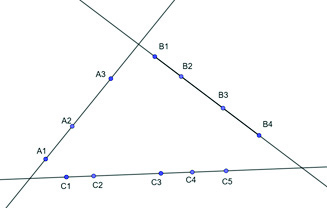
\includegraphics[width=0.4\textwidth]{10}
		%	\caption{\small\textit{Hoán vị vòng tròn $4$ người ngồi xung quanh một cái bàn hình tròn.}}
		\vspace*{-15pt}
	\end{figure}
	{Bài toán $6.2$}
	Có bao nhiêu tam giác trong hình vẽ?
	\begin{figure}[H]
		\centering
		\vspace*{-10pt}
		\captionsetup{labelformat=empty, justification=centering}
		
\includegraphics[width=0.45\textwidth]{11}
		%	\caption{\small\textit{Hoán vị vòng tròn $4$ người ngồi xung quanh một cái bàn hình tròn.}}
		\vspace*{-5pt}
	\end{figure}
	{Bài toán $6.3$}
	Có bao nhiêu tam giác được tạo bởi 3 trong 12 điểm đã cho trên lưới ô vuông như hình vẽ?
	\begin{figure}[H]
		\centering
		\vspace*{-5pt}
		\captionsetup{labelformat=empty, justification=centering}
		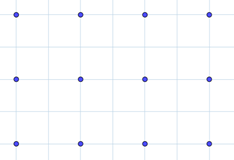
\includegraphics[width=0.4\textwidth]{12}
		%	\caption{\small\textit{Hoán vị vòng tròn $4$ người ngồi xung quanh một cái bàn hình tròn.}}
		\vspace*{-5pt}
	\end{figure}
\end{multicols}
\textbf{Bài toán số $7$: (Apmops)}
\vskip 0.1cm
Có bao nhiêu cách để tô $6$ mặt của một hình lập phương bằng $6$ mầu, mỗi mặt được tô bằng $1$ mầu sao cho không có hai mặt nào có cùng mầu? (Hai cách tô mầu được coi là như nhau nếu chúng nhìn giống hệt nhau sau một phép xoay hình). 
\vskip 0.1cm
\textbf{Phân tích bài toán:} Hướng đi thứ nhất, ta hình dung nếu cố định hình lập phương lại và mỗi cách nhìn khác nhau ở mỗi phía được coi là khác nhau, như thế thì số cách tô sẽ như tô theo hàng ngang ($6$ người ngồi trên $6$ cái ghế trên $1$ hàng) và sẽ là $6!=720$ cách. Do hình lập phương này xoay được nên ta xem mỗi một kiểu tô có bao nhiêu cách xoay nó xung quanh chính nó. Do có $6$ mầu ta có $6$ cách xuay để có đáy khác mầu. Mỗi cách đặt đáy với $1$ mầu ta có $4$ cách xoay xung quanh chính nó (do hình lập phương có $4$ cạnh bên), từ đó ta có hướng giải quyết bài toán.
\vskip 0.1cm
Hướng đi thứ $2$, do hình lập phương xoay được nên ta có thể cố định mầu ở những vị trí ta có thể xuay nó về và ta sẽ có hướng giải quyết bài toán như lời giải $2$.
\vskip 0.1cm
Hướng đi thứ $3$ gần giống với hướng thứ $2$, ta có thể hình dung mình có thể tô mầu ở đáy bằng mầu tùy thích do hình lập phương xoay được, mặt đối diện trên đỉnh sẽ còn $5$ cách tô, $4$ mặt xung quanh ta sẽ hình dung nó như $4$ người ngồi xung quanh một cái bàn tròn nên ta có thể áp dụng bài toán hoán vị vòng tròn để giải quyết.
\vskip 0.1cm
\textit{Lời giải $1$:}
\vskip 0.1cm 
Giả sử hình lập phương cố định, khi đó ta có $6!=720$ cách tô.
\vskip 0.1cm
Mỗi cách tô ta có $6$ cách đặt các mặt khác mầu nhau xuống đáy, khi đặt rồi ta có $4$ cách xoay xung quanh nó, vậy ứng với mỗi cách tô mầu ta có $6\times4=24$ cách xoay nó xung quanh chính nó. Vậy số cách tô mầu là: $720:24=30$ (cách).
\vskip 0.1cm
\textit{Lời giải $2$:}
\vskip 0.1cm 
Đầu tiên ta tô mầu $1$ mặt (mầu ta thích), rồi đặt nó xuống đáy, khi đó ở mặt đối diện trên đỉnh có $5$ cách tô.
\vskip 0.1cm
Tiếp theo ta tô mầu $1$ mặt xung quanh (mầu ta thích trong $4$ mầu còn lại), rồi xoay nó sang bên trái, khi đó mặt bên phải có $3$ cách tô, còn $2$ mặt còn lại (trước và sau) có $2!$ cách tô, vậy số cách tô mầu là: $1\times5\times1\times3\times2!=30$ (cách)
\vskip 0.1cm
\textit{Lời giải $3$:}
\vskip 0.1cm
Tương tự như lời giải $2$, đầu tiên ta tô mầu $1$ mặt (mầu ta thích), rồi đặt nó xuống đáy, khi đó ở mặt đối diện trên đỉnh có $5$ cách tô.
\vskip 0.1cm
Còn $4$ mặt xung quanh, do xoay được nên theo bài toán hoán vị vòng tròn ta có $4!/4=6$ cách tô.
\vskip 0.1cm
Vậy số cách tô mầu hình lập phương là: $5\times 6=30$ (cách).
\vskip 0.1cm
\textbf{Bài toán số $8$: (IMSO)}
\vskip 0.1cm
Một hình lập phương được tô các mặt bằng $6$ mầu, mỗi mặt $1$ mầu khác nhau và được đánh số từ $1$ đến $6$ sao cho tổng hai mặt đối diện bằng $7$. Hỏi có bao nhiêu cách tô mầu và đánh số hình lập phương này? (Hai cách tô mầu, đánh số được coi là như nhau nếu chúng nhìn giống hệt nhau sau một phép xoay hình). 
\vskip 0.1cm
Phân tích bài toán: Bài toán này là tương đối khó khi các bạn lớp $5,6$ đi thi gặp phải, và đúng là trong năm thi đó đoàn học sinh Việt Nam chỉ có đúng $1$ bạn làm được, tuy nhiên nếu chia bài toán làm hai bước, bước $1$ tô mầu, bước $2$ điền số thì ta có thể giải quyết được bài toán một cách tương đối dễ dàng.
\vskip 0.1cm
\textit{Lời giải:}
\vskip 0.1cm 
Bước $1$: Tô mầu hình lập phương, theo bài toán số $7$, ta có $30$ cách tô mầu hình lập phương này.
\vskip 0.1cm
Bước $2$: Đánh số, ta đánh theo thứ tự:
\vskip 0.1cm
Đánh số $1$, có $6$ cách. Đánh số $6$ ở mặt đối diện số $1$, có $1$ cách.
\vskip 0.1cm
Đánh số $2$, có $4$ cách (do còn $4$ mặt chưa đánh số). Đánh số $5$ ở mặt đối diện, có $1$ cách.
\vskip 0.1cm
Đánh số $3$, có $2$ cách (do còn $2$ mặt chưa đánh số). Đánh số $4$ ở mặt đối diện, có $1$ cách.
\vskip 0.1cm
Vậy ta có $6\times1\times4\times1\times2\times1=48$ cách đánh số.
\vskip 0.1cm
Theo quy tắc nhân ta có số cách tô mầu và đánh số là: $30\times 48=1440$ (cách).
\vskip 0.1cm
\begin{multicols}{2}
	\textbf{Bài toán số $9$: (IMAS)}
	\vskip 0.1cm
	Một bàn cờ hình vuông $5\times 5$ được xếp một hình chữ L chiếm $4$ ô như hình vẽ. Ta có thể xuay hoặc lật hình chữ L này. Hỏi có bao nhiêu cách xếp hình chữ L này vào bàn cờ hình vuông đã cho?
	\begin{figure}[H]
		\centering
		\vspace*{-5pt}
		\captionsetup{labelformat=empty, justification=centering}
		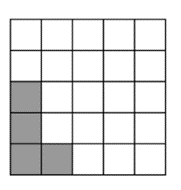
\includegraphics[width=0.4\textwidth]{13}
		%	\caption{\small\textit{Hoán vị vòng tròn $4$ người ngồi xung quanh một cái bàn hình tròn.}}
		\vspace*{-5pt}
	\end{figure}
\end{multicols}
Phân tích bài toán: Ta nhận thấy hình chữ L tô đen có thể xoay hoặc lật được, nên ta sẽ xem nó có thể có bao nhiêu cách biến hình (xoay hoặc lật).  Ứng với mỗi phép biến hình bằng xoay, lật ta xem có bao nhiêu cách trượt nó theo hàng ngang và hàng dọc, từ đó ta có cách giải quyết bài toán.
\vskip 0.1cm
\textit{Lời giải:}
\vskip 0.1cm
Ta tính số cách xoay, lật hình chữ L tô đậm, như hình dưới ta có $8$ cách.
	\begin{figure}[H]
	\centering
	\vspace*{-5pt}
	\captionsetup{labelformat=empty, justification=centering}
	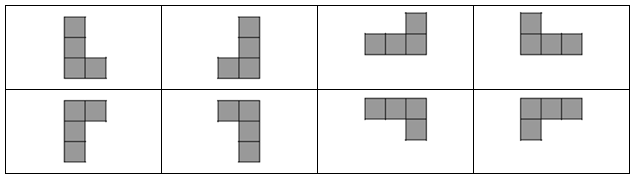
\includegraphics[width=1\textwidth]{14}
	%	\caption{\small\textit{Hoán vị vòng tròn $4$ người ngồi xung quanh một cái bàn hình tròn.}}
	\vspace*{-15pt}
\end{figure}
Ứng với mỗi cách biến hình này, ta xem có bao nhiêu cách dời hình theo hàng ngang và hàng dọc, và ta tính được số cách dời hình bằng trượt (tịnh tiến) theo hai chiều ngang, dọc là: $3\times4=12$.
\begin{multicols}{2}
		\begin{figure}[H]
		\centering
		\vspace*{-5pt}
		\captionsetup{labelformat=empty, justification=centering}
		
\includegraphics[width=0.5\textwidth]{15}
		%	\caption{\small\textit{Hoán vị vòng tròn $4$ người ngồi xung quanh một cái bàn hình tròn.}}
		\vspace*{-15pt}
	\end{figure}
	Theo quy tắc nhân, ta có số cách đặt chữ L vào ô vuông $5\times 5$ là: $8\times12=96$ (cách)
\end{multicols}
Mở rộng bài toán số $9$. Các bạn thử sức mình xem nhé.
\vskip 0.1cm
Bài toán số $9.1$: Đề bài giống như bài toán số $9$, hình được xếp vào được thay đổi như sau:
	\begin{figure}[H]
	\centering
	\vspace*{-5pt}
	\captionsetup{labelformat=empty, justification=centering}
	
\includegraphics[height=0.4\textwidth]{16}\quad
	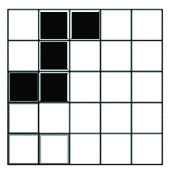
\includegraphics[height=0.4\textwidth]{17}
	\caption{\small\textit{$a)$ \hspace*{130pt} $b)$}}
	\vspace*{-15pt}
\end{figure}
\textbf{Bài toán số $10$: (IMSO).}
\vskip 0.1cm
Một hình tròn và một tam giác được xếp trên các điểm cắt của lưới ô vuông như hình vẽ sao cho tam giác và hình tròn không cùng nằm trên một hàng hay một cột.
\vskip 0.1cm
\begin{multicols}{2}
	Hỏi có bao nhiêu cách xếp tam giác và hình tròn vào lưới ô vuông như hình vẽ này. Trên hình vẽ là một ví dụ về cách xếp tam giác và hình tròn.
	\begin{figure}[H]
		\centering
		\vspace*{-25pt}
		\captionsetup{labelformat=empty, justification=centering}
		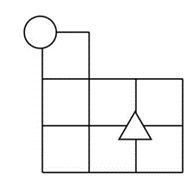
\includegraphics[width=0.4\textwidth]{18}
		\vspace*{-5pt}
	\end{figure}
\end{multicols}
\textbf{Phân tích bài toán:} Bài toán này các bạn nhỏ lớp $4,5$ trong câu lạc bộ toán UMC đã làm được theo nhiều cách khác nhau, các bạn quan sát sẽ thấy ngoài hai điểm ở hàng trên cùng thi bên dưới cứ mỗi hình chữ nhật sẽ có $2!\times 2!=4$ cách đặt hình tròn và tam giác (do mỗi cặp đỉnh không kề nhau của $1$ hình chữ nhật sẽ có $2!$ cách đặt hình tròn và tam giác). Sau đây là một số cách giải của các bạn.
\vskip 0.1cm
\textit{Lời giải $1$: }(Lê Kỳ Nam, Vĩnh Giang)
\vskip 0.1cm
Nếu đường tròn nằm trên hàng đầu tiên (có $2$ vị trí), thì ở mỗi vị trí sẽ có $14 - 4 - 1 = 9$ cách chọn tam giác, tổng số cách chọn là: $9 \times 2 = 18$.
\vskip 0.1cm
Nếu đường tròn đi vào phần còn lại của $2$ cột đầu tiên, thì ở mỗi vị trí, số cách chọn tam giác là $14 - 3 - 3 - 1 = 7$, tổng số cách chọn là $6 \times 7 = 42$.
\vskip 0.1cm
Nếu đường tròn đi ở $2$ cột cuối cùng, thì ở mỗi vị trí, tam giác sẽ có $14 - 3 - 2 - 1 = 8$ lựa chọn, tổng số cách chọn là $6 \times 8 = 48$.
\vskip 0.1cm
Tổng số cách xếp hình tròn và hình tam giác là: $18 + 42 + 48 = 108$.
\vskip 0.1cm
Đáp số: $108$
\vskip 0.1cm
\textit{Lời giải $2$:} (Nguyễn Gia Tuấn)
\vskip 0.1cm
Nếu hình tròn và hình tam giác không được đặt trên hình vuông trên cùng thì có $3 \times 4 \times 2 \times 3 = 72$ cách chọn.
\vskip 0.1cm
Nếu một trong các tam giác hoặc hình tròn được đặt trên hình vuông trên cùng thì có $2 \times 3 \times 3 \times 2 = 36$ cách chọn.
\vskip 0.1cm
Tổng cộng có $72 + 36 = 108$ cách chọn.
\vskip 0.1cm
\textit{Lời giải $3$:} (Nguyễn Trọng Cường).
\vskip 0.1cm
Tổng số các cách có thể đặt hình tròn và tam giác vào $2$ điểm bất kỳ của hình là: $14\times13 = 182$ cách
\vskip 0.1cm
Nếu hình tròn và tam giác nằm trên cùng $1$ cột, hoặc $1$ hàng, thì $2$ điểm sẽ tạo nên $1$ đoạn thẳng. Ta đếm số đoạn thẳng của hình trên.
\vskip 0.1cm
Số đoạn thẳng của hình là :
\begin{align*}
	1 + (1+2+3) \times 3 + (1+2+3) \times 2 + (1+2) \times 2 = 37
\end{align*}
Hình tròn và tam giác ở $2$ đầu đoạn thẳng, đổi chỗ được cho nhau $\Rightarrow$ có $37 \times 2 = 74$ cách ko thỏa mãn
\vskip 0.1cm
Số cách thỏa mãn đề bài là $182 - 74 = 108$ cách.
\vskip 0.1cm
\textit{Lời giải $4$:} (Nguyễn Gia Tuấn). -- Dùng phần bù:
\vskip 0.1cm
Với lưới ô vuông $3 \times 3$ thì ta có $C(4,2)\times C(4,2)\times 4 = 144$ cách chọn. (Do mỗi hình chữ nhật có $4$ cách đặt tam giác và hình tròn).
\vskip 0.1cm
Trong lưới $3 \times 3$ đó, nếu đặt hình tròn hoặc tam giác vào $2$ điểm trên cùng ở bên phải thì có $2 \times 3 \times  3 \times 2 = 36$ cách chọn.
\vskip 0.1cm
Vậy ta có $144 - 36 = 108$ cách chọn để xếp hình tròn và hình tam giác.
\vskip 0.1cm
Trả lời: $108$ lựa chọn.
